\newpage
\setcounter{page}{1}
\section{Project description}

\subsection{Research background}

In this section, we briefly summarize the state-of-the-art in the proposed
research areas and outline the current state of the principal investigator own
research.

\subsubsection{Current state of research in the field}
Since the first introduction of Bitcoin, the demand for blockchain solutions is
increasing over the years. There exist a multitude of blockchain technologies since
then, try to address different aspects of digital life. In the core of most
blockchains, essentially, assets are transferred under the control of custom
scripts (so-called \emph{smart contracts}) that enforce necessary conditions to
transfer an asset from one party to another. Being the first generation of
blockchain, Bitcoin has very limited support for smart contracts. On the other
hand, later generations of blockchain (Ethereum, NEO, Stellar, etc.) address
this problem by providing a general-purpose programmable infrastructure, where
the blockchain does not only store financial data but also have the capability
of deploying and executing custom code on the blockchain system. For example,
Ethereum is after Bitcoin the second-largest cryptocurrency platform by market
capitalization. Unlike Bitcoin, Ethereum supports programmable smart contracts
with an entire programming language along with it, running in Ethereum Virtual
Machine (EVM) \cite{ethereum:evm}. The flexibility within a smart contract
allows users to implement their own autonomous execution logic on blockchains
enable more options for optimization. However, several challenges in blockchain
technology remain to be addressed, two of which are scalability and
interoperability.

\paragraph*{Scalability} The performance of mainstream blockchains is still a
barrier to the adoption of blockchain technology. As a global payment system,
Visa is capable of processing around 24,000 transactions per second on average
\cite{visa}, while Bitcoin and Ethereum can handle 7 and 15 transactions per
second \cite{ethereum:sharding, nakamoto2019bitcoin}. Scaling the performance of
blockchain systems has become a hot topic for both industry and academia, with
many proposals. Those proposals vary from optimizing the performance of the
consensus protocols \cite{dang2019towards}, partitioning the blockchain
\cite{wang2019sok}, to shifting the computation from the blockchain (on-chain)
to the outside (off-chain) \cite{teutsch2019scalable, network2018cheap}. Among
all the proposed methods for scaling the performance, sharding the blockchain state
is an effective and practical solution, as it can overcome both performance and
scalability problems of blockchain. Partitioning (or \emph{sharding}) is a
technique that divides the state of a service or a system in multiple partitions
so that most requests or transactions access one partition only and are equally
distributed among partitions (e.g., \cite{facebookTAO, sciascia2012sdur,
aguilera2007sinfonia}). As a result, partitions can work in parallel to maximize
performance and improve throughput. In the context of blockchain, state
partitioning is challenging, however, due to fundamental differences between
previous domains and blockchain, notably the failure model. With its
decentralized nature, there is no single entity in a blockchain system that
contains information of all objects in the network, which makes it difficult for
blockchain clients to locate objects in the presence of partitioning. RapidChain
\cite{zamani2018rapidchain} builds a routing overlay network for users and
committee leaders to locate the committee where to send their transactions.
Moreover, with the lacking of overall information, choosing a partition to place
the objects in order to maximize the balance between partitions is not
effective. Even if enough information is available, finding a good partitioning
is a complex optimization problem~\cite{curino2010sch,taft2014est}. To the best
of our knowledge, no work has focused on achieving an optimized partitioning for
blockchain sharding.

\paragraph*{Interoperability} With the increasing number of blockchain systems
and distributed applications (DApps), there is a rising demand for
interoperability. Interoperability in the context of blockchain means connecting
multiple blockchains to share, exchange, or changing the state of the own or the
other blockchain \cite{buterin2016chain}. In the recent evolvement of blockchain
technologies, some blockchain systems have supported interoperability in their
core, in the form of an inter blockchain communication (IBC) protocol
\cite{kwon2016cosmos, thomas2015protocol, kokoris2018omniledger,
al2017chainspace}. Moreover, some solutions start to appear that allows smart
contracts to move between existing blockchains \cite{fynn2020move,
back2014enabling, herlihy2018atomic}. In \cite{fynn2020move}, Fynn \emph{et al.}
introduced a move primitive \cite{fynn2020move} allows programmable blockchains
to interoperate by moving contracts and data from one to another. The
possibilities of interoperability are endless. An application in a private
blockchain can access data from a public blockchain \cite{prusty2018blockchain},
A contract can shift an expensive computational off-chain
\cite{teutsch2019scalable, network2018cheap}, or a DApps can access data from
multiple blockchains. However, it also leaves new open questions. One could be
how to locate objects in a blockchain, while contracts and objects are being
moved around, or is it financially beneficial to move a calculation to a
side-chain.

\subsubsection{Current state of principal investigator's research}

Investigator Long Hoang Le conducts research in distributed systems. Much of his
work has focused on scalable and faults tolerant system, particularly in scaling
state machine replication \cite{le2016dssmr, le2019dynastar, bezerra2016strong}.
His work on DS-SMR \cite{le2016dssmr} was nominated for best paper award at DSN
2016. 

State machine replication is a common approach to building fault-tolerant
systems \cite{Lam78, Sch90}. Participants in a replicated state machine system
form agreement on a sequence of transactions and apply them in sequence order
deterministically to reach the same state. With its simple yet effective
execution model, state machine replication is at the core of many blockchain
systems \cite{baudet2019state, cachin2016architecture}. This approach provides a
configurable degree of availability but limits the achievable throughput of the
replicated service to what a single replica can process sequentially. In the
work \dynastar \cite{le2019dynastar}, Le \emph{et al.} proposed an approach for
scaling the performance of SMR by allowing the SMR system to partition the state and
reconfigure its data placement on-the-fly. \dynastar maintains a location oracle
with a global view of the application state. Figure \ref{fig:tpcc} shows the
performance evaluation of \dynastar with TPC-C benchmark. Figure
\ref{fig:tpcc}(a) depicts the impact of partitioning on the performance of a
system before and after an optimized partitioning configuration is applied.
Figure \ref{fig:tpcc}(b) shows the scalability of \dynastar when increase the
size of the system (adding more data and computational resources). This result
suggests that by using the data of the oracle to come up with an optimized
partitioning, scalable performance for SMR is achievable for real-world
application.

It's worth it to
 note that in a TPC-C benchmark, the average rate of multi-partition transactions
 is 15\

\begin{figure*}[ht!]
  \centering
  \begin{subfigure}{.48\textwidth}
    \centering
    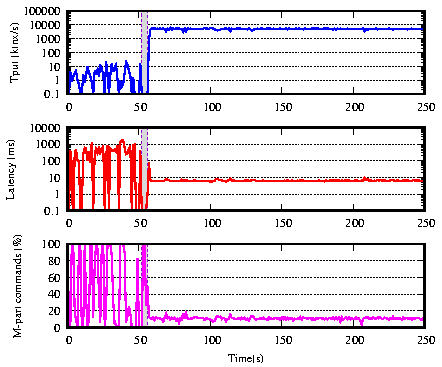
\includegraphics[width=0.8\columnwidth]{figures/tpcc-detail-dynastar}
  \caption{Repartitioning in \dynastar; throughput (top), objects exchanged
  between partitions (middle), and percentage of multi-partition commands
  (bottom).}
  \end{subfigure}
  \begin{subfigure}{.48\textwidth}
    \centering
    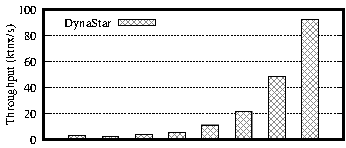
\includegraphics[width=\textwidth]{./figures/tpcc-scaling-tp-lat-bridge}
    \caption{Performance scalability with TPC-C. Throughput (in thousands of transactions per second, ktps)}
  \end{subfigure}
  \caption{Performance of Dynastar with TPC-C Benchmark}
  \label{fig:tpcc}
\end{figure*}

\subsection{Innovation potential and market review} 

This project's main goal is to develop an oracle service that analyzes
blockchain's transactions to provide such necessary information. The service
will answer several questions such as where are the objects or contracts
after they have been moved across different blockchain, where to put the objects
to optimize the partitioning of the network to improve the performance, or to
which side-chain off-load a transaction is financially beneficial.

The information provided by our oracle service serves multiple purposes. First,
it provides a location mapping for contracts and objects within and across
partitions. This enables blockchain clients to quickly locate to which
partitions or blockchain they should send their transactions. Second, the
location mapping opens up possibilities for further improvements, e.g.,
computing the optimized location for the upcoming transactions and object.
Third, with the information of the execution cost and time provided by our
oracle service, the blockchain client can decide to off-load expensive
computation to a side-chain to optimize the cost.

% With the on-chain component in the form of smart contract, our proposed system
% could be integrated to existing blockchain systems easily without any change in
% the blockchain protocol. 

% In an analysis in \cite{fynn2020move}, the author performed an extensive study
% on the impact of partitioning Ethereum blockchain. The study showed that even on
% a workload that was not created for a sharded system, an optimized partitioning
% scheme could achieve a rate of less than ten percents of cross partition
% transaction. 

Figure \ref{fig:transaction-fee} shows the mean value in USD of transaction
fee in the first six months of the year 2020 \cite{transactionfee}. This data
suggests that the average fee for executing an ordinary transaction in Stellar
network is 1,000 times cheaper than on Ethereum Classic network, and is 100,000
times cheaper than running on Ethereum. If this information is available at the
time of execution, the blockchain can make an effective decision of where to
execute the transaction. However, it does make two important assumptions: (i)
the transaction is executable on all parties (i.e., there is a smart contract of
this transaction type available on both blockchains). (ii) there exists a move
operation that could send the necessary data from one contract to another (such
primitive was proposed in \cite{fynn2020move}).

\begin{figure*}[ht!]
\begin{minipage}[b]{1\linewidth}
\centering
      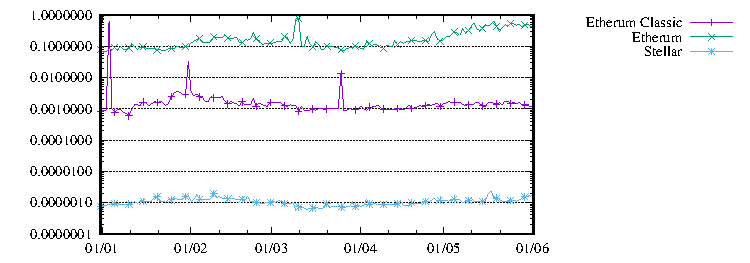
\includegraphics[width=0.6\linewidth]{figures/transaction-fee-mean-usd}
\end{minipage}
\caption{Transaction fee of Ethereum, Ethereum Classic and Stellar in USD value in first half of 2020}
\label{fig:transaction-fee}
\end{figure*}

\subsection{Implementation strategy}
\label{sec:strategy}
Figure \ref{fig:architecture} presents the overall architecture of the
proposed oracle service. The core components of the system are divided in two
parts: the on-chain smart contract component and the off-chain service
component. The on-chain smart contract (OSC) is a set of smart contracts that
are developed separately for each supported blockchain. The OSC plays the roles
of the interface of the service, receives requests from other contracts in the
form of contract calls, and dispatches those requests to the off-chain component.
The OSC is also responsible for computing the fee of each request. The off-chain
component consists of a computational unit (CU) and a set of blockchain
analyzers. The analyzers monitor the blockchains by actively fetching and
analyzing the transaction history to aggregate multiple metrics of a standard
blockchain, for example, the location of contracts and objects in the case of
movement, the average execution cost, or the pending transactions count, etc. The
CU is a set of computational nodes that serves requests by historical data
fetched by the analyzers. Upon receiving requests from user smart contract, the
OSC validates the requests and forwards those requests to the CU. The CU queries
the data from the backlog and replies to the OSC. Once receiving the response from CU,
the OSC calculates the fee for the request, and send back the data to the user
smart contract.

\begin{figure*}[ht!]
\begin{minipage}[b]{1\linewidth}
\centering
      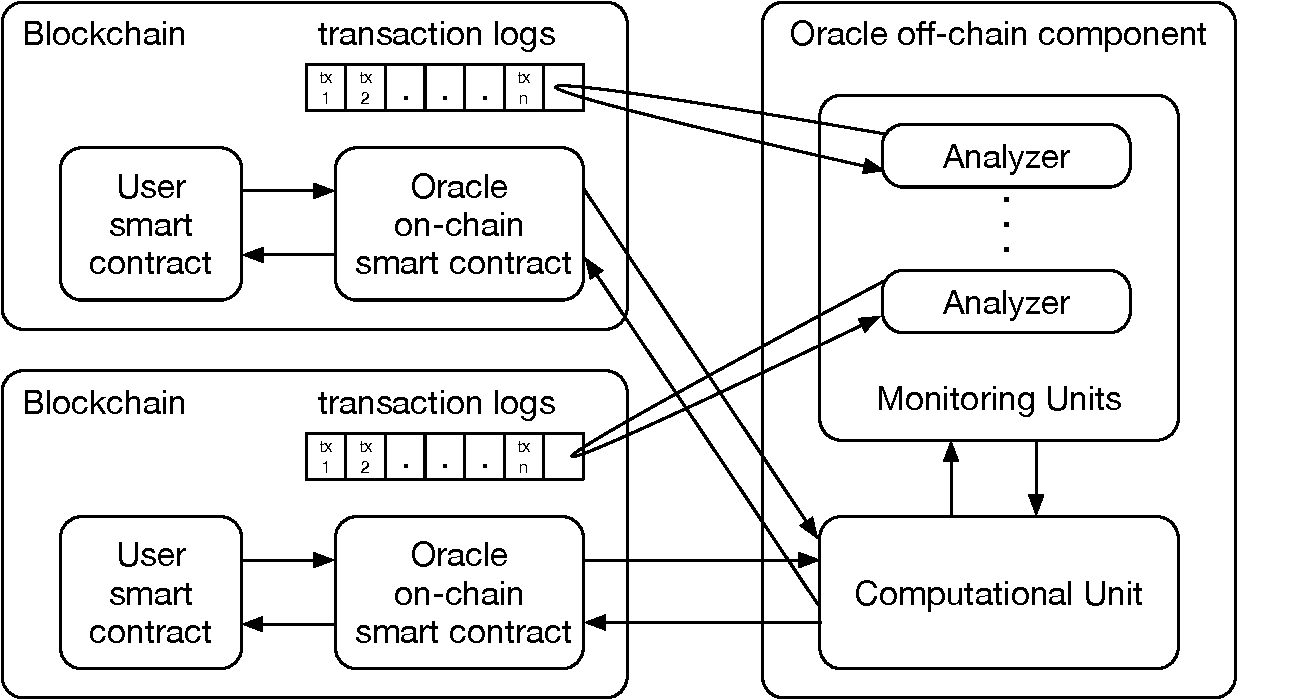
\includegraphics[width=0.6\linewidth]{figures/architecture}
\end{minipage}
\caption{The architecture of the proposed oracle service}
\label{fig:architecture}
\end{figure*}

\subsection{Project plan}

The project plan will divide the research activities described in Section
\ref{sec:strategy} into three phases. Figure \cite{fig:plan} identifies the major
milestones for each of the activity areas, as well as milestones for the overall
system evaluation.

% \paragraph*{Research Goal 1}
% \emph{Implementing on-chain smart contracts.}

% \begin{description}
%   \item \textbf{Tasks}
%   \item RG1T1. Develop an abstraction for blockchain analyzers
%   \item RG1T2. Implementing at least two analyzers for two sample blockchains
%   \item RG1T3. Implementing the computational unit
% \end{description}

% \begin{description}
%   \item \textbf{Milestones}
%   \item RG1M1. Blockchain analyzers implementation
%   \item RG1T2. Computational unit implementation
% \end{description}


% \paragraph*{Research Goal 2}
% \emph{Developing on-chain smart contracts.}

% \begin{description}
%   \item \textbf{Tasks}
%   \item RG2T1. Develop an abstraction for the on-chain smart contract
%   \item RG2T2. Implementing at least two smart contracts for two sample blockchains
% \end{description}

% \begin{description}
%   \item \textbf{Milestones}
%   \item RG2M1. On-chain smart contract implementation
% \end{description}


% \paragraph*{Research Goal 3}
% \emph{Integrating and evaluating}

% \begin{description}
%   \item \textbf{Tasks}
%   \item RG3T1. Deploy all components for supported blockchains
%   \item RG3T2. Developing benchmark decentralized application
%   \item RG3T3. Evaluating the effectiveness of the service
% \end{description}

% \begin{description}
%   \item \textbf{Milestones}
%   \item RG3M1. Benchmark DApps implementation
%   \item RG3M2. All components of the service are deployed
% \end{description}

\begin{figure*}[ht!]
  \begin{minipage}[b]{1\linewidth}
  \centering
        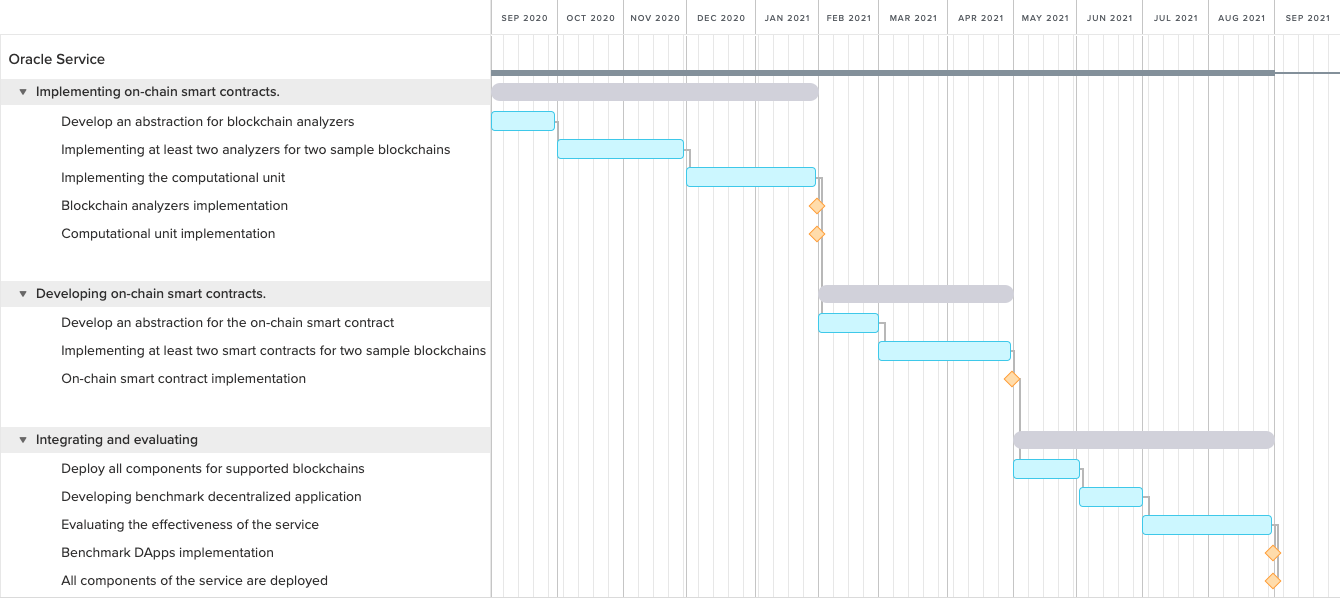
\includegraphics[width=1\linewidth]{figures/plan-details.png}
  \end{minipage}
  \caption{A tentative project timetable.}
  \label{fig:plan}
  \end{figure*}
  
% Information of blockchains, including historical data of transaction, execution
% fee, execution delay, etc can be fetched and monitored by analyzers....


